%%%%%%%%%%%%%%%%%%%%%%%%%%%%%%%%%%%%%%%%%
% Short Sectioned Assignment
% LaTeX Template
% Version 1.0 (5/5/12)
%
% This template has been downloaded from:
% http://www.LaTeXTemplates.com
%
% Original author:
% Frits Wenneker (http://www.howtotex.com)
%
% License:
% CC BY-NC-SA 3.0 (http://creativecommons.org/licenses/by-nc-sa/3.0/)
%
%%%%%%%%%%%%%%%%%%%%%%%%%%%%%%%%%%%%%%%%%

%----------------------------------------------------------------------------------------
%	PACKAGES AND OTHER DOCUMENT CONFIGURATIONS
%----------------------------------------------------------------------------------------

\documentclass[paper=a4, fontsize=11pt]{scrartcl} % A4 paper and 11pt font size

\usepackage[T1]{fontenc} % Use 8-bit encoding that has 256 glyphs
\usepackage{fourier} % Use the Adobe Utopia font for the document - comment this line to return to the LaTeX default
\usepackage[english]{babel} % English language/hyphenation
\usepackage{amsmath,amsfonts,amsthm} % Math packages

\usepackage{lipsum} % Used for inserting dummy 'Lorem ipsum' text into the template

\usepackage{sectsty} % Allows customizing section commands
\allsectionsfont{\centering \normalfont\scshape} % Make all sections centered, the default font and small caps

\usepackage{tikz}
\usetikzlibrary{plotmarks}

\usepackage{enumitem}
\usepackage{lastpage}
\usepackage{multirow}
\usepackage{fancyhdr} % Custom headers and footers
\pagestyle{fancyplain} % Makes all pages in the document conform to the custom headers and footers
\fancyhead{} % No page header - if you want one, create it in the same way as the footers below
\fancyfoot[L]{} % Empty left footer
\fancyfoot[C]{} % Empty center footer
\fancyfoot[C]{\thepage~of~\pageref{LastPage}} % Page numbering for right footer
\renewcommand{\headrulewidth}{0pt} % Remove header underlines
\renewcommand{\footrulewidth}{0pt} % Remove footer underlines
\setlength{\headheight}{13.6pt} % Customize the height of the header

\setlength\parindent{0pt} % Removes all indentation from paragraphs - comment this line for an assignment with lots of text

%----------------------------------------------------------------------------------------
%	TITLE SECTION
%----------------------------------------------------------------------------------------

\newcommand{\horrule}[1]{\rule{\linewidth}{#1}} % Create horizontal rule command with 1 argument of height



\title{	
\normalfont \normalsize 
\textsc{Norwegian University of Science and Technology\\TDT4200 -- Parallel Computing} \\ [25pt]
\horrule{0.5pt} \\[0.4cm]
\huge Problem Set 1:\\ MPI Intro\\
\horrule{2pt} \\[0.5cm]
}

\author{Per Magnus Veierland\\permve@stud.ntnu.no}

\setlist[enumerate,1]{label=\emph{\alph*})}
\setlist[enumerate,2]{label=\roman*)}
\setlist[enumerate,3]{label=\arabic*)}

\date{\normalsize\today}

\begin{filecontents}{div_soft.data}
#MOPS   Power [mW]
1.33E-02    10.403432
1.33E-01    12.53108
2.66E-01    14.90265
3.99E-01    17.22483
5.31E-01    19.58292
6.64E-01    21.89876
7.97E-01    24.44624
9.30E-01    26.6708
\end{filecontents}

\begin{document}
\maketitle

\section*{Part 1: Theory}

\subsection*{Problem 1: General Theory}

\begin{enumerate}

\item \textbf{Write a table explaining Flynn’s Taxonomy.}

\begin{table}
\begin{center}
\begin{tabular}{c|cc}
& \multicolumn{2}{|c}{Instruction Stream}\\
\hline
\multirow{2}{*}{Data Stream} & Single & Multiple\\
& Single & Multiple\\
\end{tabular}
\end{center}
\end{table}

\begin{enumerate}

\item \textbf{Explain how, where, and why MPI fits into Flynn's Taxonomy, and why if not.}

\end{enumerate}

\item \textbf{Shared Memory}

\begin{enumerate}

\item \textbf{Explain how and why (and why if not), MPI fits with Shared Memory systems.}

\end{enumerate}

\item \textbf{Distributed Memory}

\begin{enumerate}

\item \textbf{Explain how and why (and why if not), MPI fits with Distributed Memory systems.}

\end{enumerate}

\end{enumerate}

\subsection*{Problem 2: Code Theory}

\begin{enumerate}

\item \textbf{Does your implementation have any communicational bottlenecks?}

\begin{enumerate}

\item \textbf{Briefly outline the communicational bottleneck(s), if any.}

\item \textbf{Is it possible to reduce the bottleneck, and if so how?}

\begin{enumerate}

\item \textbf{If so, outline an algorithm that will reduce the bottleneck.}

\end{enumerate}

\end{enumerate}

\item \textbf{Does your implementation have any computational bottlenecks?}

\begin{enumerate}

\item \textbf{Briefly outline the computational bottleneck(s), if any.}

\item \textbf{Is it possible to reduce the bottleneck(s)?}

\begin{enumerate}

\item \textbf{If so, outline an algorithm/method that will reduce the bottleneck.\\A one line formula, if found, is acceptable (this is a hard question).}

\end{enumerate}

\end{enumerate}

\end{enumerate}

\section*{Part 2: Code}

\subsection*{Problem 1: MPI Intro}

\begin{enumerate}

\item \textbf{In the MPI copy \texttt{computeMPI.c}, parallelize the serial program from \texttt{computeSerial.c} using MPI.}

\item \textbf{Implement a ``make all'' Makefile-rule which compiles and executes corresponding MPI file/executable in the given Makefile.}

\item \textbf{Analyze your implementation and report the following:}

\begin{enumerate}

\item \textbf{The amount of operations performed by your program as a function of $O(n)$, $n = stop - start$, and the amount of operations performed per process $\text{P}_\text{i}$ in your program with $i \in [1, 10]$.}

\item \textbf{The amount of MPI operations performed by your program as a function of $O(P)$, $P = NumberOfProcesses$.}

The program is split into one master process communicating with a set of slave processes. Each slave process will perform its computation based on the command line inputs and send one result to the master process using \texttt{MPI\_Send}. The number of slave processes is $P - 1$.

The master process will perform its own computation based on the command line inputs and then receive one result from each slave process using \texttt{MPI\_Recv}.

In total, the number of MPI operations performed by the program will be two times the number of slave processes; since each \texttt{MPI\_Send} from each slave process must be matched by one \texttt{MPI\_Recv} by the master process. Accordingly, $O(P) = P$.
$$\textit{NumberOfMpiOperations} = 2 * \textit{NumberOfSlaveProcesses} = 2 * (P - 1) = 2P - 2$$
$$O(P) = P$$

\item \textbf{The average amount of MPI operations performed per process $\text{P}_\text{i}$ in your program with $O(P)$, $P = NumberOfProcesses$.}

$(2P - 2) / P$

\item \textbf{The maximum number of MPI operations performed by any process $\text{P}_\text{i}$ as a function of $O(P)$, $P = NumberOfProcesses$.}

Will be by master node:
$P - 1$

\item \textbf{The difference in run-time with $P \in [1, 2, 4, 8]$ and $n = [2 \to 100, 2 \to 10^6, 2 \to 10^9]$ when run on a machine in ITS015.\\Make a graph for each value of P, showing the run-time for different increments of n. Each range of n should be split into 20 steps of equal increments.}

% format

% 4 graphs for each P



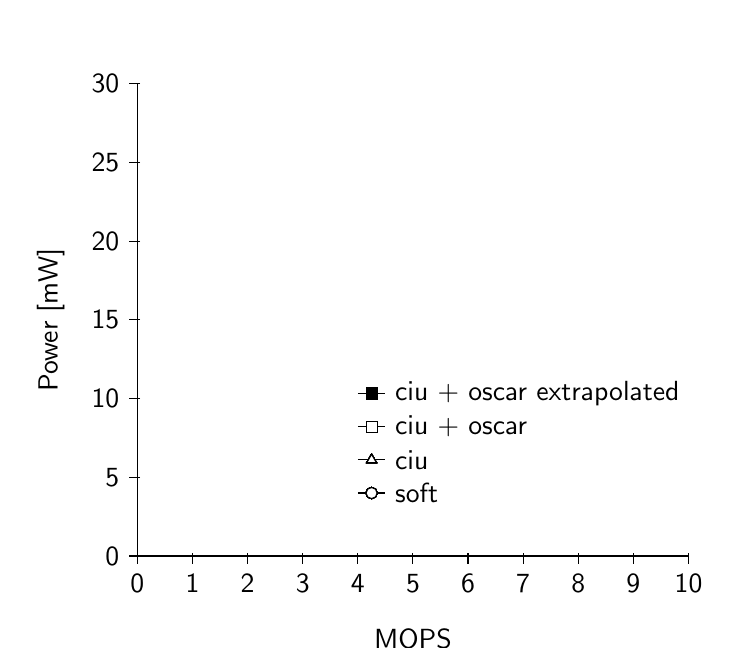
\begin{tikzpicture}[y=.2cm, x=.7cm,font=\sffamily]
%axis
\draw (0,0) -- coordinate (x axis mid) (10,0);
\draw (0,0) -- coordinate (y axis mid) (0,30);
%ticks
\foreach \x in {0,...,10}
\draw (\x,1pt) -- (\x,-3pt)
node[anchor=north] {\x};
\foreach \y in {0,5,...,30}
\draw (1pt,\y) -- (-3pt,\y) 
node[anchor=east] {\y}; 
%labels      
\node[below=0.8cm] at (x axis mid) {MOPS};
\node[rotate=90, above=0.8cm] at (y axis mid) {Power [mW]};

%plots
\draw plot[mark=*, mark options={fill=white}] 
file {div_soft.data};

%legend
\begin{scope}[shift={(4,4)}] 
\draw (0,0) -- 
plot[mark=*, mark options={fill=white}] (0.25,0) -- (0.5,0) 
node[right]{soft};
\draw[yshift=\baselineskip] (0,0) -- 
plot[mark=triangle*, mark options={fill=white}] (0.25,0) -- (0.5,0)
node[right]{ciu};
\draw[yshift=2\baselineskip] (0,0) -- 
plot[mark=square*, mark options={fill=white}] (0.25,0) -- (0.5,0)
node[right]{ciu + oscar};
\draw[yshift=3\baselineskip] (0,0) -- 
plot[mark=square*, mark options={fill=black}] (0.25,0) -- (0.5,0)
node[right]{ciu + oscar extrapolated};
\end{scope}
\end{tikzpicture}

\end{enumerate}

\end{enumerate}

\end{document}

